\documentclass[aspectratio=169, plain, 14pt]{beamer}
\beamertemplatenavigationsymbolsempty
\setbeamertemplate{footline}[frame number]
\usepackage[utf8]{inputenc}
\usepackage[russian]{babel}
\usepackage[table]{xcolor}
\setbeamertemplate{itemize items}[circle]
\usepackage{ragged2e}
\usepackage{mathtools}
\usepackage{cleveref}
\usepackage{physics}

%My blocks
\setbeamercolor{block title}{fg=white,bg=blue!65!black}
\setbeamercolor{block body}{fg=black,bg=blue!10!white}
%%%%%%%%%%%%%%%%%%%%%%%%%%%%%%%%%%%

\title{Л3. Модель аэродинамических сил и моментов}
\author{Сутурин Даниил}
\institute{ЦНИИХМ}
\date{\today}

\begin{document}
\begin{frame}
    \titlepage{}
\end{frame}
%%%%%%%%%%%%%%%%%%%%%%%%%%%%%%%%%%%%%%
\begin{frame}{Обзор}
\large
    \begin{itemize}
    \item Уравнения движения твердого тела
    \item Общий вид ЛА
    \item Модель аэродинамических сил
    \item Модель аэродинамических моментов
    \end{itemize}
\end{frame}
%%%%%%%%%%%%%%%%%%%%%%%%%%%%%%%%%%%%%%%%%%%%%%%%%%%%%%%%%%
\begin{frame}{Вектор состояния. Напоминание}
\only<1>{
\small
\begin{center}
    \begin{tabular}{|m{0.5cm}||m{13cm}|}
        \hline
        \rowcolor{lightgray} \multicolumn{2}{|c|}{\textbf{Фазовые переменные ЛА}}\\
        \hline\hline
        $p_{n}$ & Положение ЛА по северной координате $x_i$ в NED \\
        \hline
        $p_e$ & Положение ЛА по восточной координате $y_i$ в NED \\
        \hline
        $p_d$ & Положение ЛА по вертикальной координате $z_i$  в NED \\
        \hline
        $\phi$ & крен \\
        \hline
        $\theta$ & тангаж \\
        \hline
        $\psi$ & рыскание \\
        \hline
        $u$ & компонента скорости ЛА относительно  земли вдоль $x_b$ ССК \\
        \hline
        $v$ & компонента скорости ЛА относительно земли вдоль $y_b$ ССК \\
        \hline
        $w$ & компонента скорости ЛА относительно земли вдоль $z_b$ ССК \\
        \hline
        $p$ & Компонента угловой скорости ЛА $\omega_{b/i}^b$ вдоль $x_b$ ССК \\
        \hline
        $q$ & Компонента угловой скорости ЛА $\omega_{b/i}^b$ вдоль $y_b$ ССК \\
        \hline
        $r$ & Компонента угловой скорости ЛА $\omega_{b/i}^b$ вдоль $z_b$ ССК \\
        \hline
        
    \end{tabular}
\end{center}
}
%%%%%%%%%%%%%%%%%%%%%%%%%%%%%%%%%%%%%%%%%%%%%%%%%%%%%%%%%
\only<2>{
\small\justifying
Необходимо определить, каким образом фазовые переменные, определенные выше в таблице, зависят от друг друга, от внешних условий среды, параметров летательного аппарата (размер, масса, двигательная установка и т.д.):

$$\dot{\boldsymbol{x}} = \begin{pmatrix}
    \dot{p_n}\\ \dot{p_e}\\ \dot{p_d}\\\dot{\phi}\\\dot{\theta}\\:\\
\end{pmatrix} = \boldsymbol{f}(\boldsymbol{x}, \boldsymbol{u})$$
где $\boldsymbol{x}$ - вектор состояния, $\boldsymbol{u}$ - вектор управления
}
\end{frame}
%%%%%%%%%%%%%%%%%%%%%%%%%%%%%%%%%%%%%%%%%%%%%%%%%%%%%%%%%
\begin{frame}{Уравнения движения. Напоминание}
\only<1>{
    $$\begin{pmatrix}
        \dot{p_n}\\\dot{p_e}\\\dot{p_d}\\
        \dot{u}\\\dot{v}\\\dot{w}\\
        \dot{\phi}\\\dot{\theta}\\\dot{\psi}\\
        \dot{p}\\\dot{q}\\\dot{r}
    \end{pmatrix} 
    =
    \begin{pmatrix}
        (R_i^b)^T\begin{pmatrix}
            u\\v\\w
        \end{pmatrix}\\
        
        \frac{1}{m}\begin{pmatrix}
        f_{x_{b}}\\f_{y_{b}}\\f_{z_{b}}
        \end{pmatrix} + \begin{pmatrix}
            rv - qw \\ pw-ru \\qu-pv
        \end{pmatrix}\\

        H(\boldsymbol{\Phi})\begin{pmatrix}
            p\\q\\r
        \end{pmatrix}\\

        J^{-1}[\begin{pmatrix}
            M_{x_{b}}\\M_{y_{b}}\\M_{z_{b}}
        \end{pmatrix} - \boldsymbol{\omega}_{b/i}^b\times(J\boldsymbol{\omega}_{b/i}^b)]
    \end{pmatrix}$$
    }
%%%%%%%%%%%%%%%%%%%%%%%%%%%%%%%%%%%%%%%%%%%%%%%%%%%
\only<2>{
	\justifying\small
	Уравнения выше описывают поступательное и вращательное движение любого твердого тела относительно некоторой инерциальной системы координат. Специфика конкретного объекта заложена в моделях сил $\boldsymbol{f^b} = (f_{x_b} \quad f_{y_b} \quad f_{z_b})^T$ и моментов сил $\boldsymbol{M^b} = (M_{x_b} \quad M_{y_b} \quad M_{z_b})^T$, действующих на тело. 
}
\end{frame}

%%%%%%%%%%%%%%%%%%%%%%%%%%%%%%%%%%%%%%%%%%%%%%%%%%%%%%%
\begin{frame}{Конфигурация крыла}
\only<1>{
\small
Существует множество аэродинамических схем ЛА, включающие различные расположения и формы крыла, хвостового оперения, количества управляющих поверхностей и положения двигателя. Всевозможные комбинации этих вариантов приводят к огромному количеству конфигураций ЛА и, как следствие, к разным динамическим свойствам
}
%%%%%%%%%%%%%%%%%%%%%%%%%%%%%%%%%%%%%%%%%%%%%
\only<2>{
\begin{figure}
    \centering
    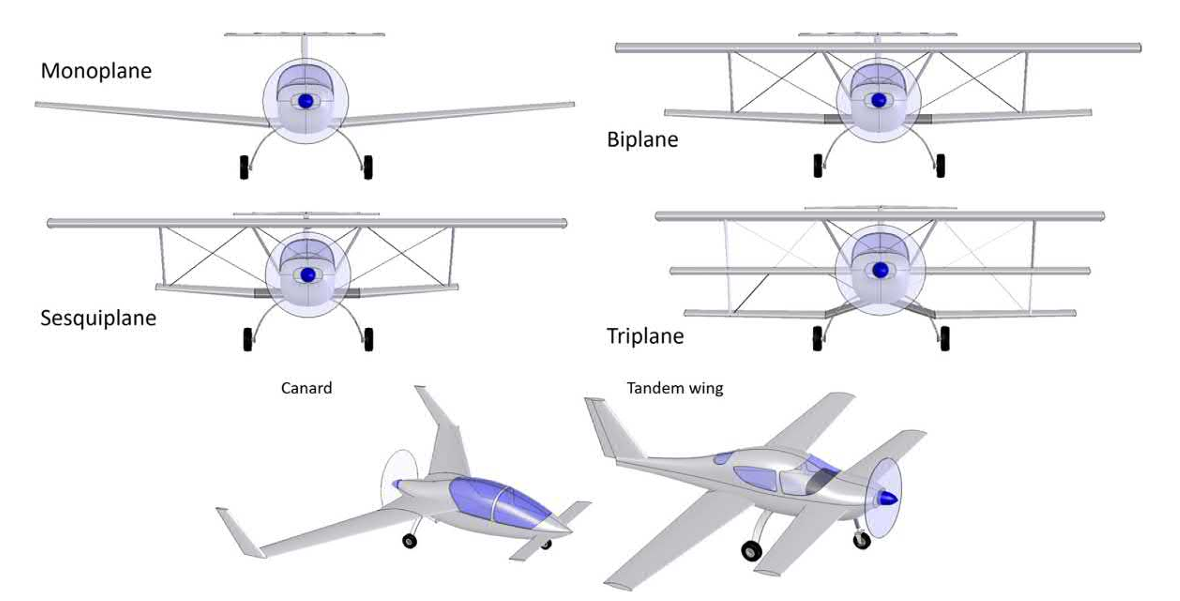
\includegraphics[width=1\linewidth]{WingConf.png}
\end{figure}
}
\end{frame}
%%%%%%%%%%%%%%%%%%%%%%%%%%%%%%%%%
\begin{frame}{Конфигурация хвостового оперения}
    \begin{figure}
    \centering
    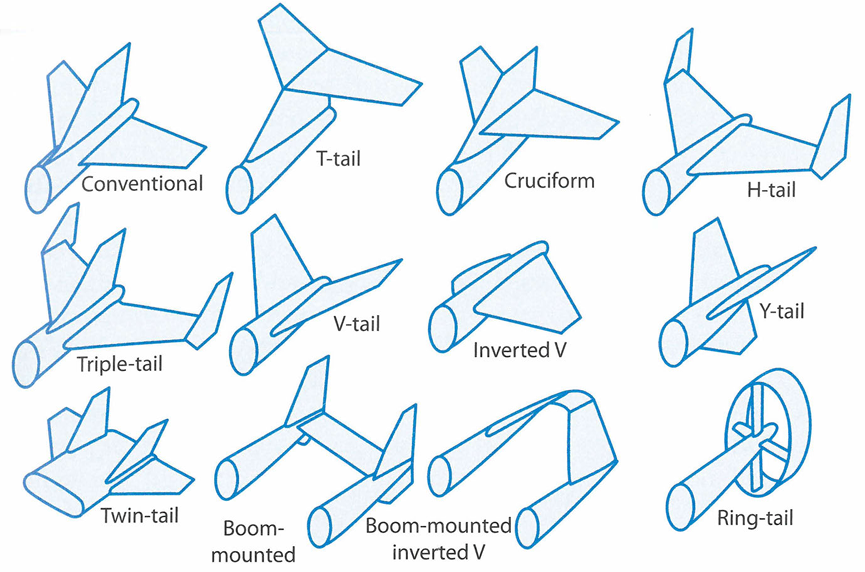
\includegraphics[width=0.8\linewidth]{TailConf.png}
\end{figure}
\end{frame}
%%%%%%%%%%%%%%%%%%%%%%%%%%%%%%%%%%%%%%%%
\begin{frame}{Расположение двигателя}
    \begin{figure}
    \centering
    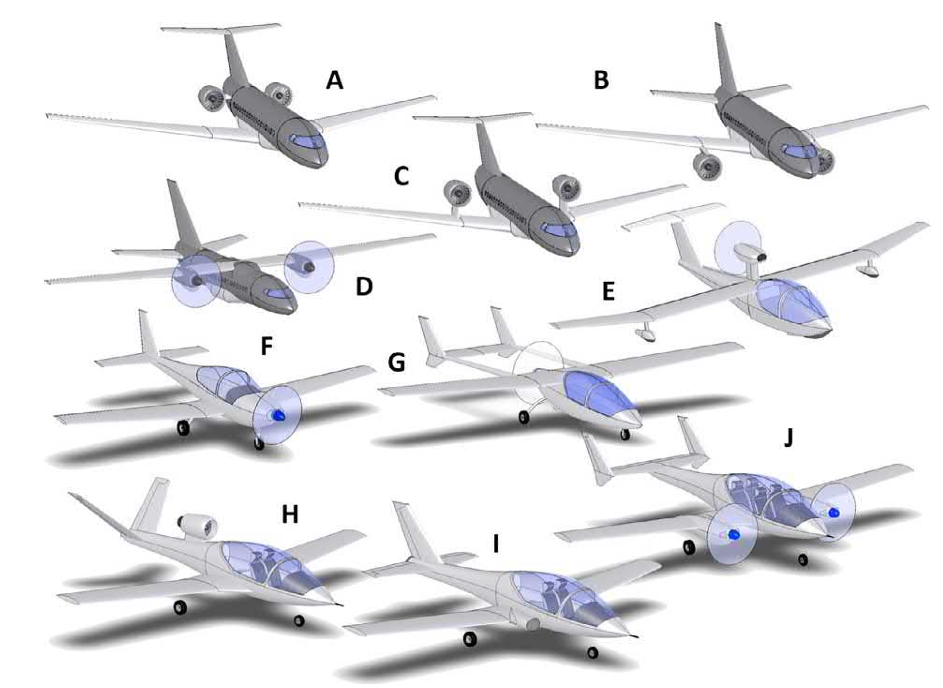
\includegraphics[width=0.8\linewidth]{EngieConf.png}
\end{figure}
\end{frame}
%%%%%%%%%%%%%%%%%%%%%%%%%%%%%%%%%%%%%%%%
\begin{frame}{Элементы конструкции ЛА}
\only<1>{
    \begin{figure}
    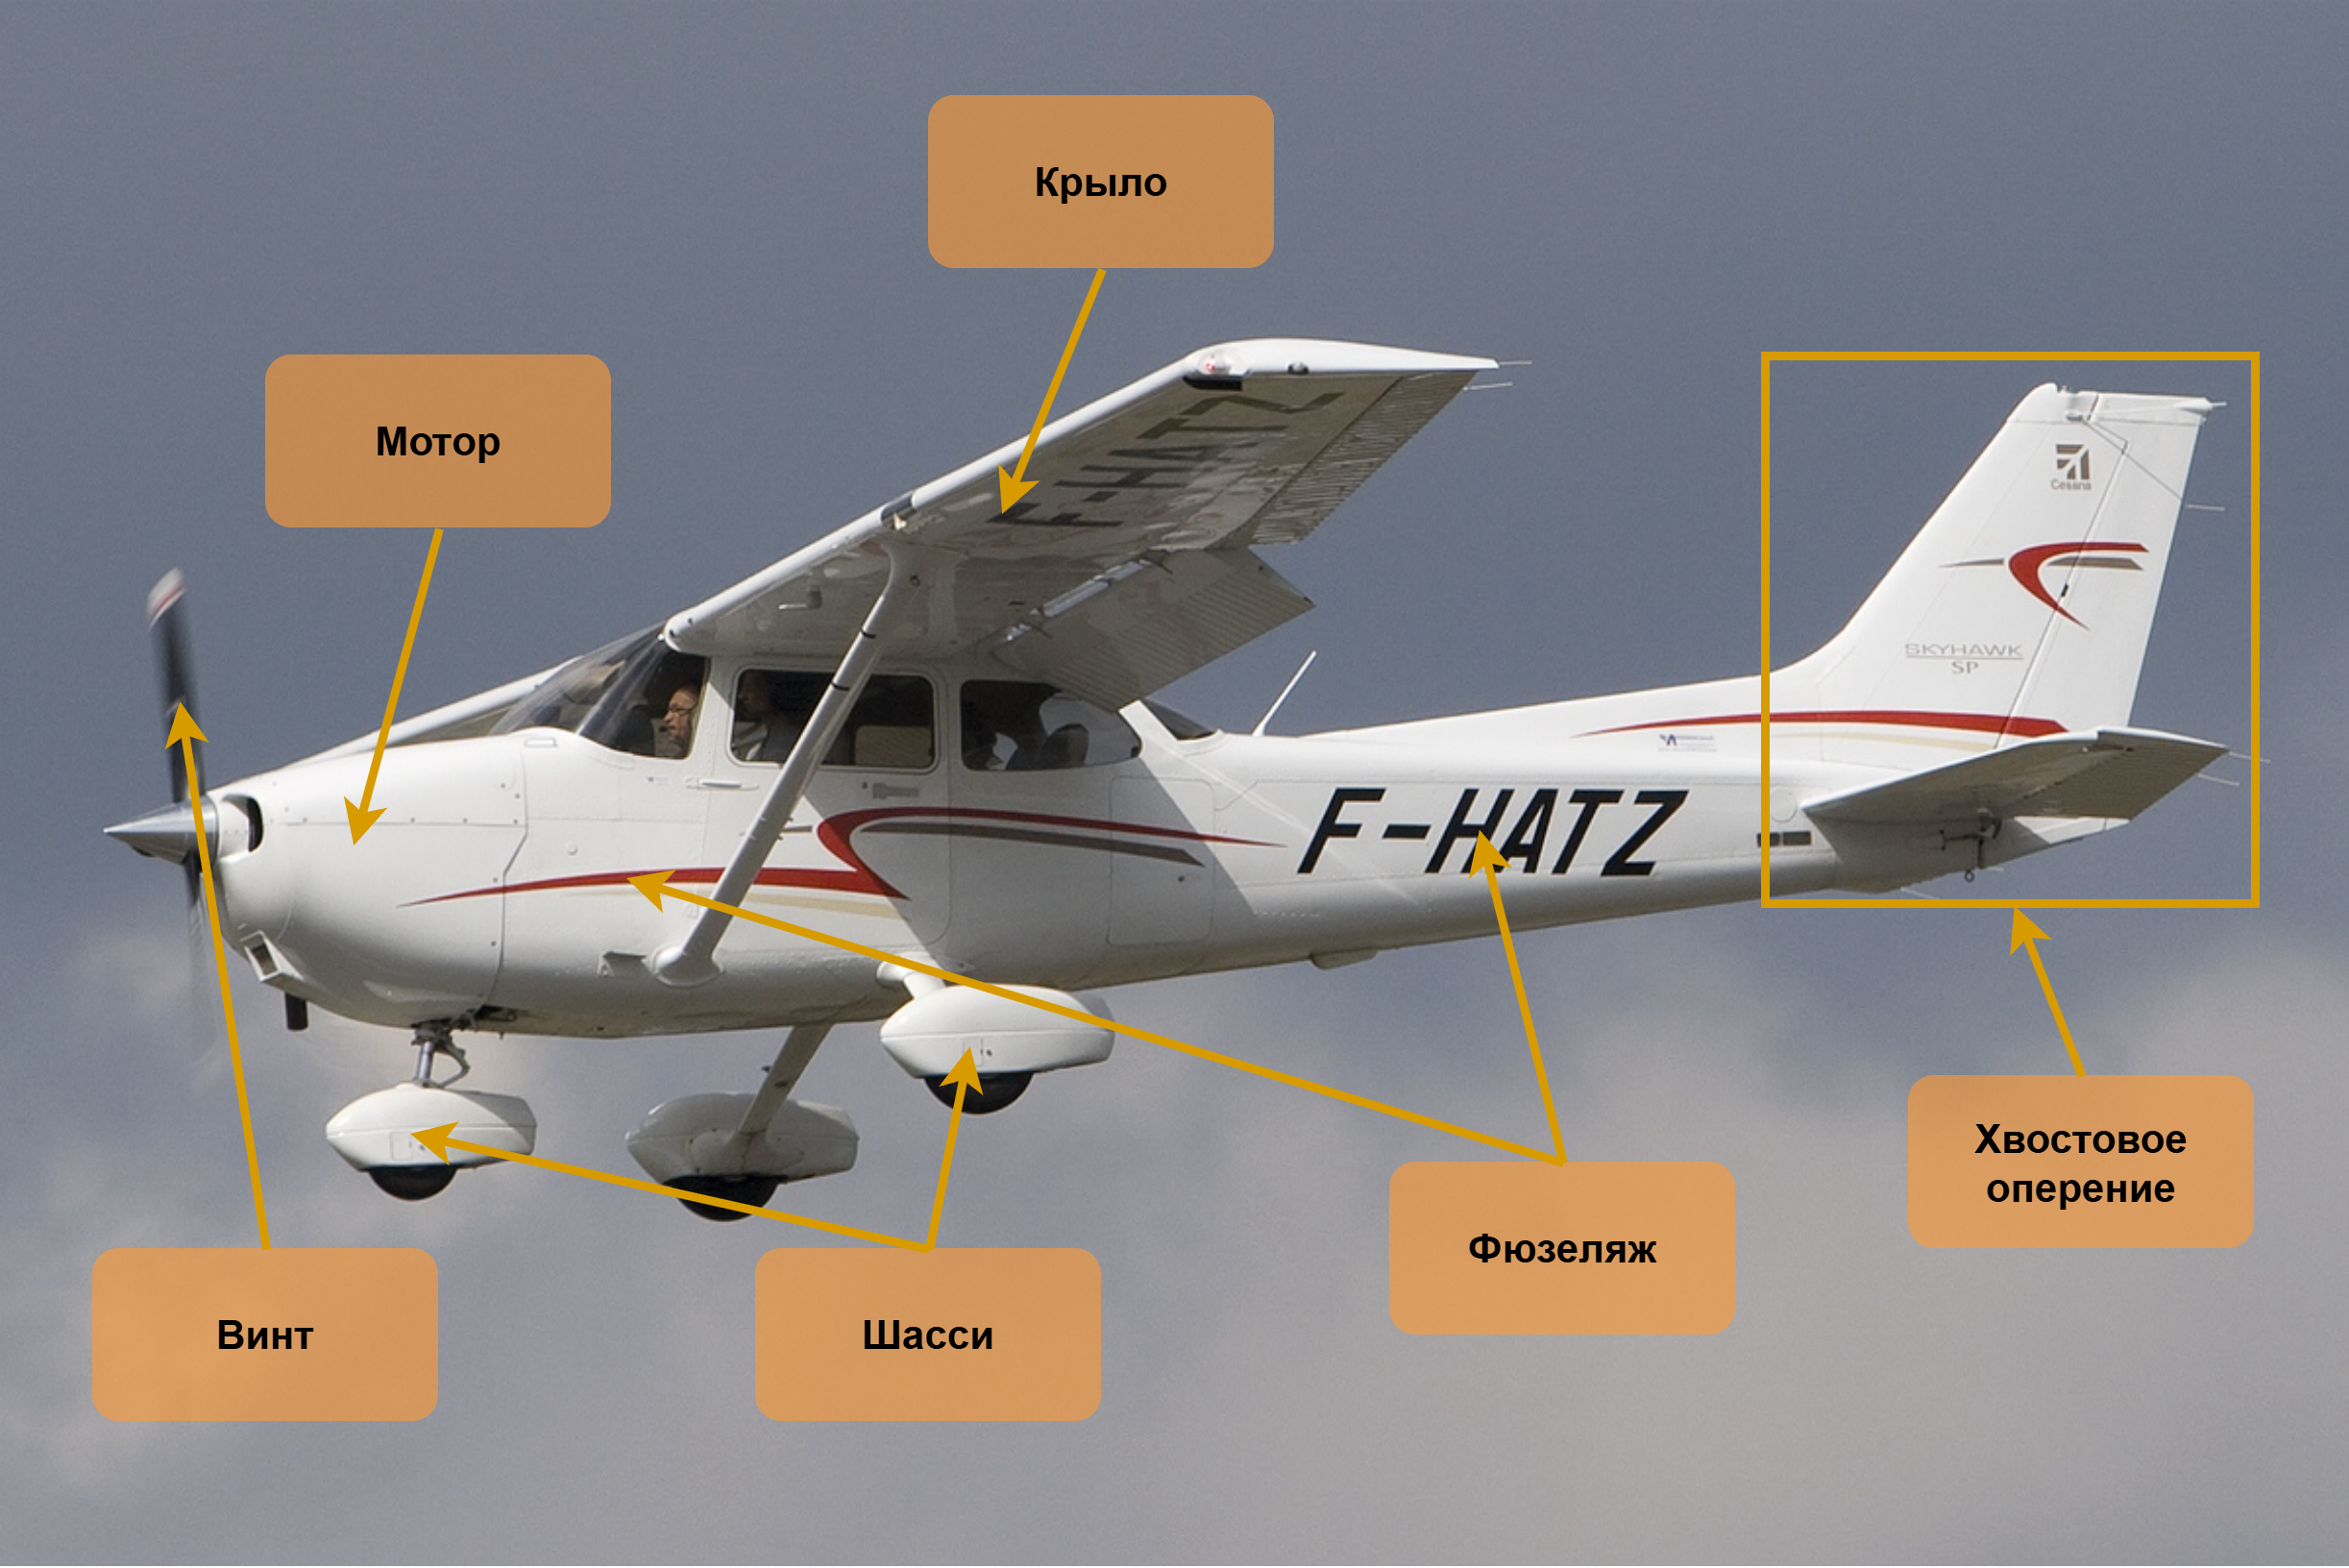
\includegraphics[width=0.8\linewidth]{PlaneGenView.png}
    \end{figure}
}
\only<2>{
    \begin{figure}
    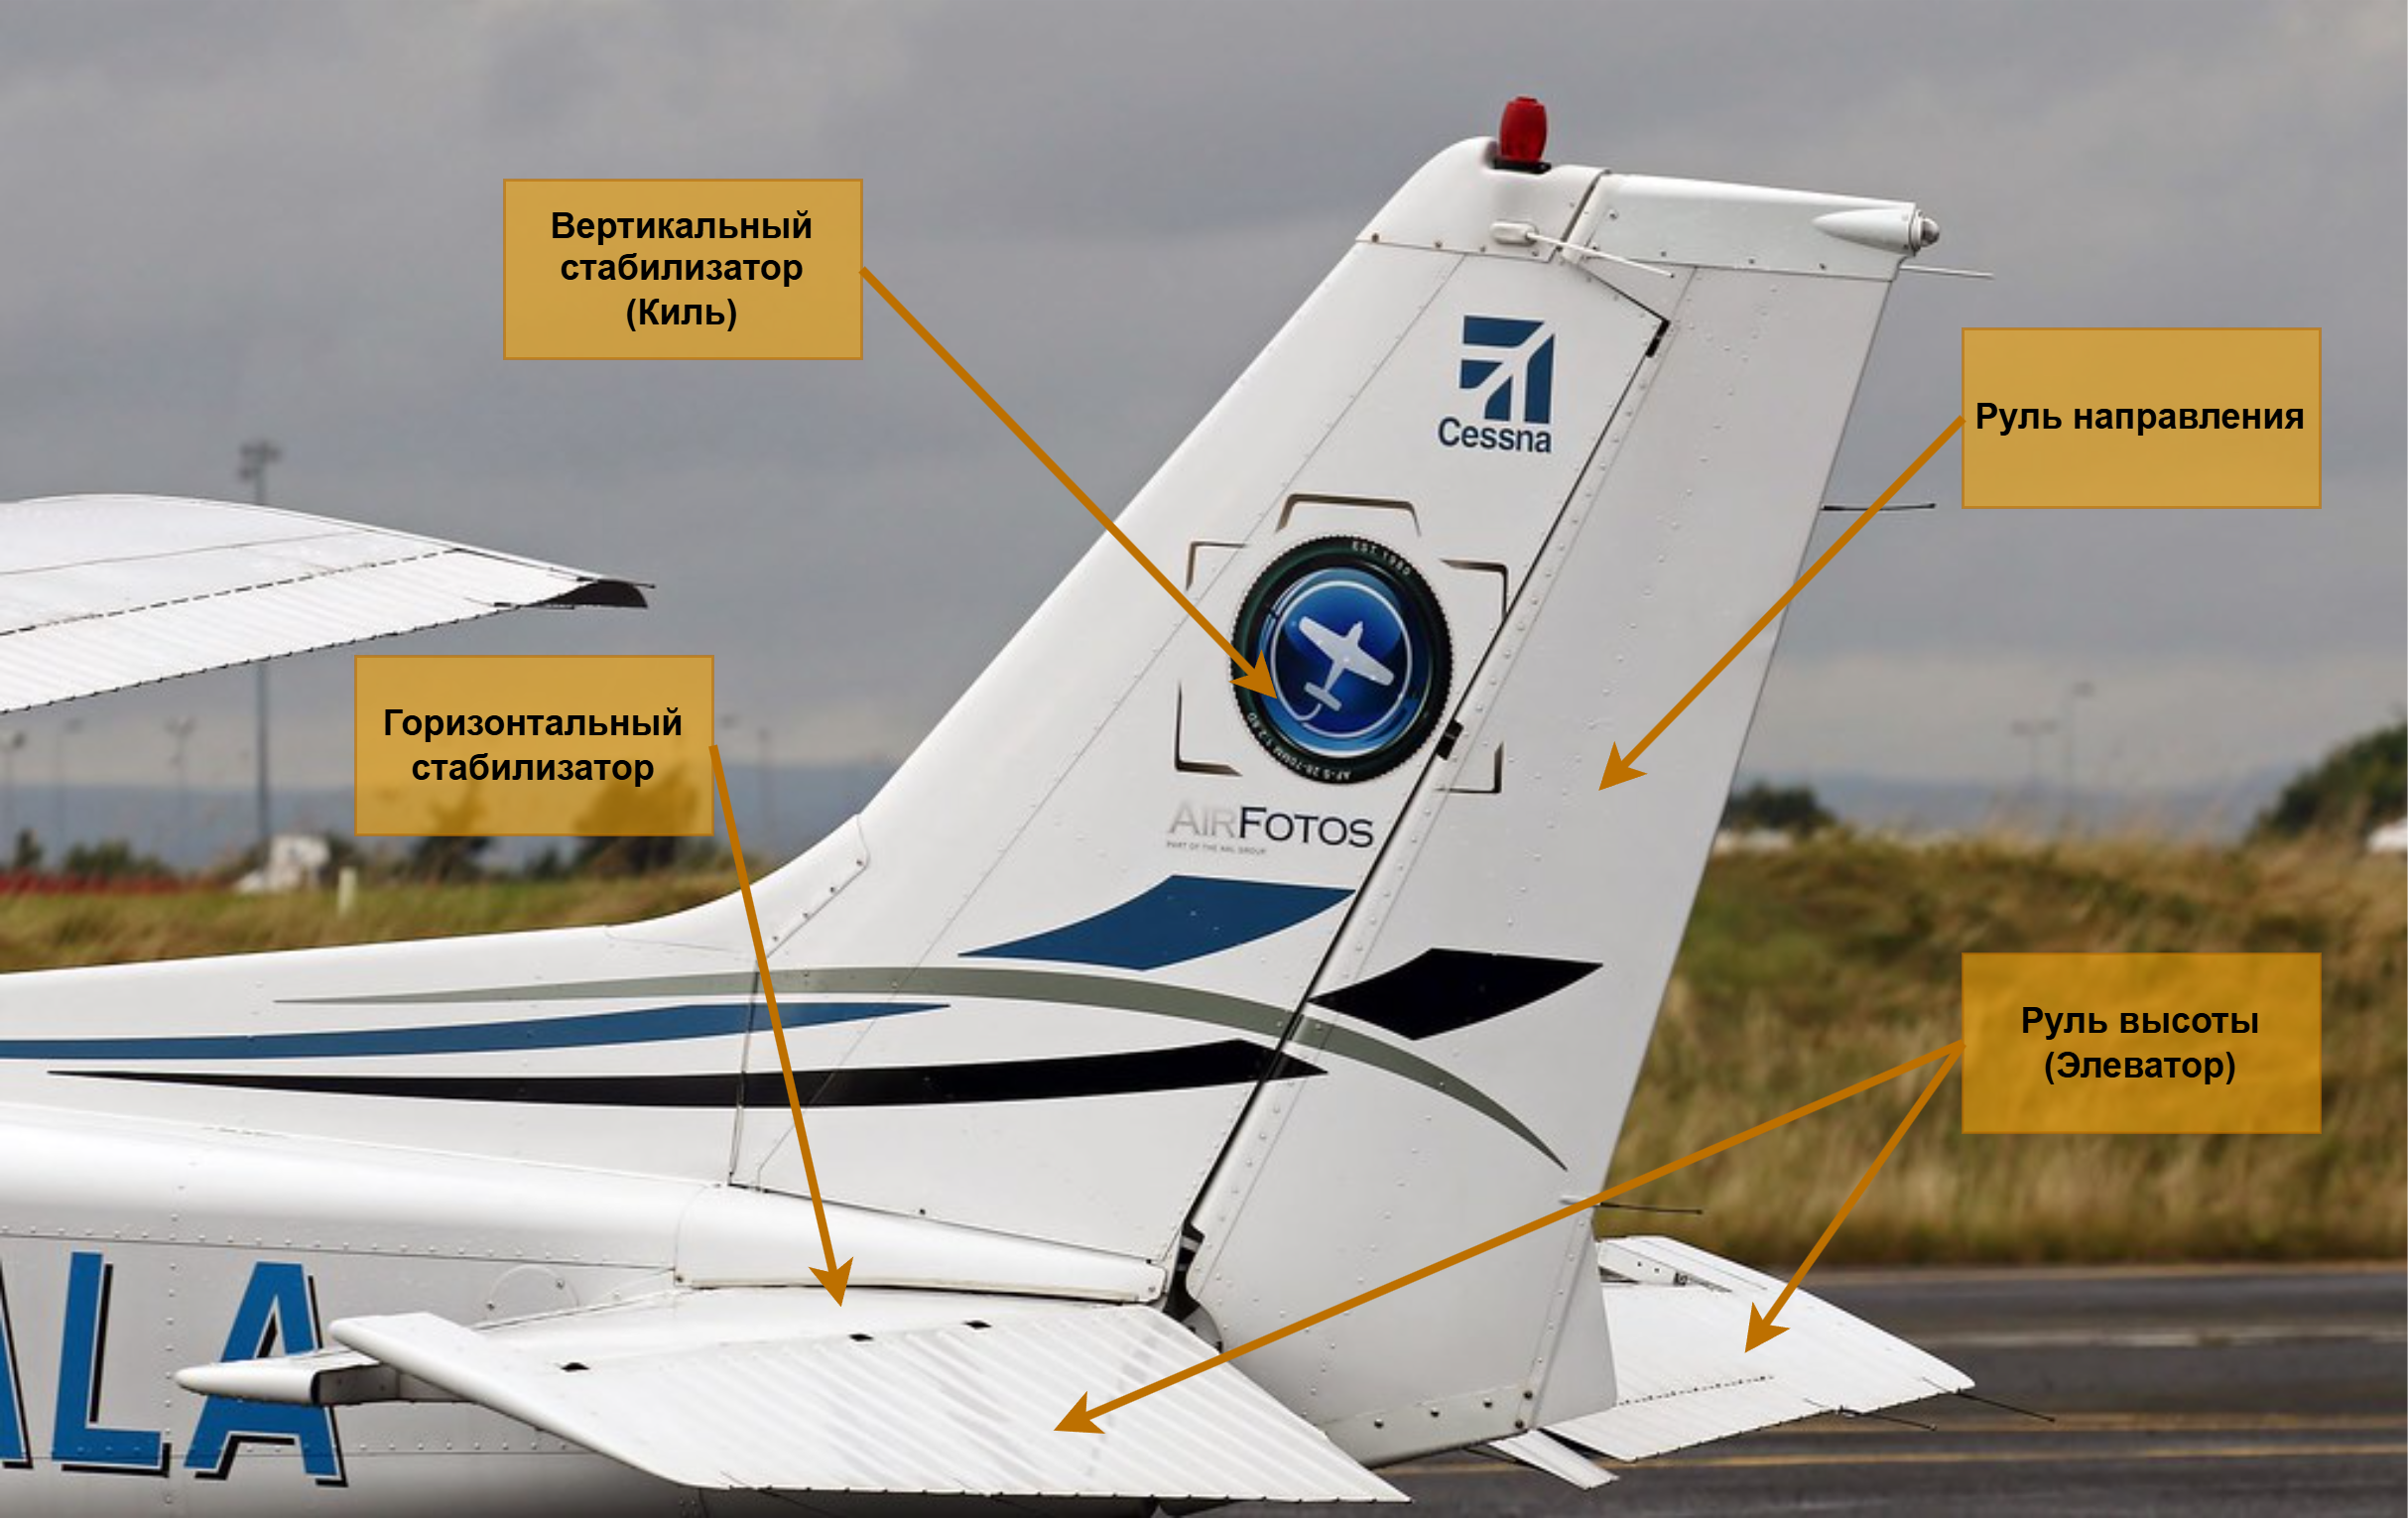
\includegraphics[width=0.8\linewidth]{PlaneTailView.png}
    \end{figure}
}
\only<3>{
    \begin{figure}
    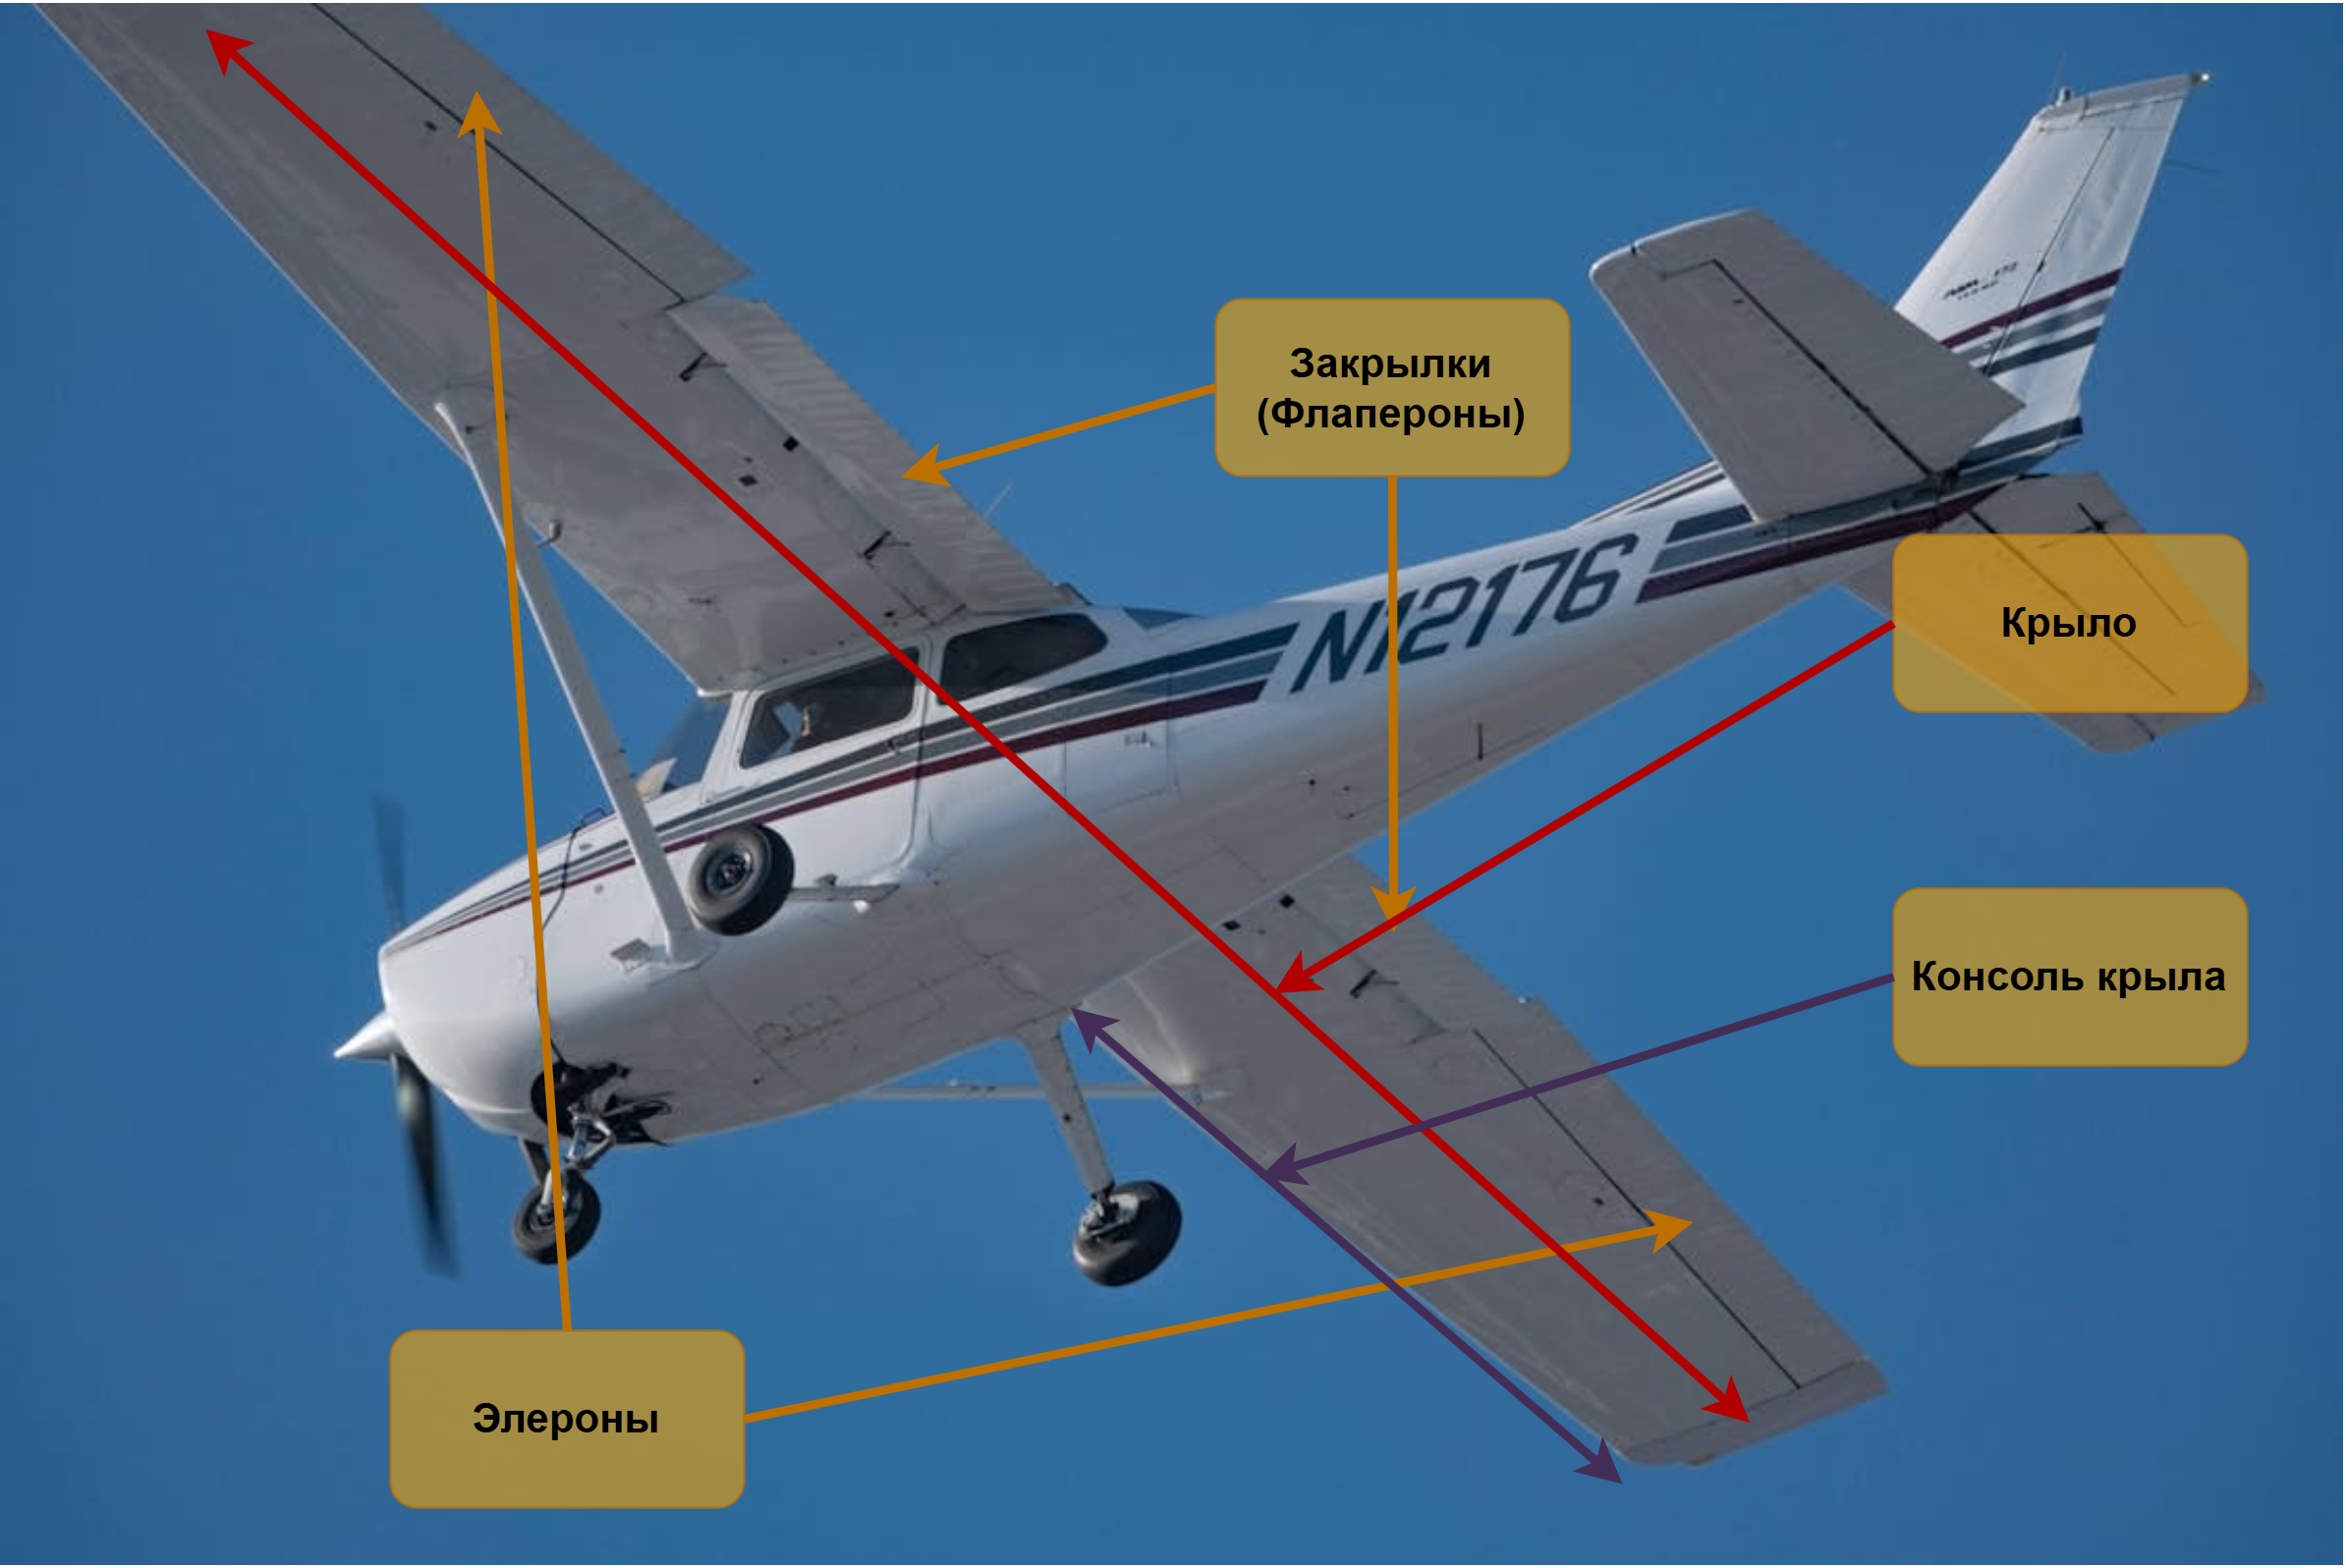
\includegraphics[width=0.8\linewidth]{PlaneBottomView.png}
    \end{figure}
}
\end{frame}
%%%%%%%%%%%%%%%%%%%%%%%%%%%%%%%%%%%%%%%%%%%%%%%%%%%%%%%%%%%
\begin{frame}{Модель ЛА}
	\small\justifying
	
	\begin{columns}
	\column{0.5\textwidth}
		\begin{figure}
		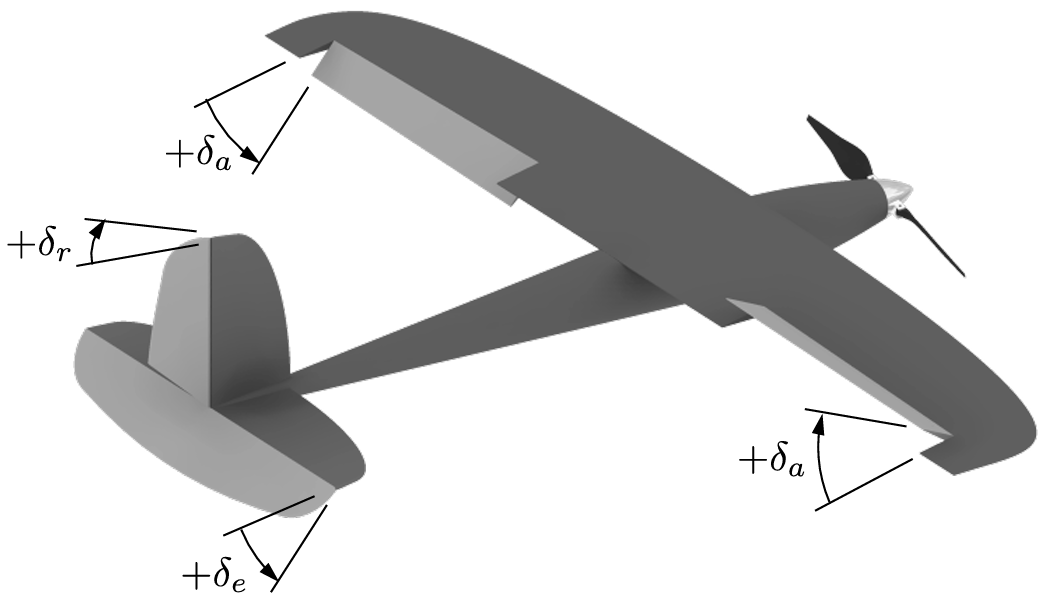
\includegraphics[width=1\linewidth]{ControlSurfaces.png}
		\end{figure}
	
	\column{0.5\textwidth}
		Будем рассматривать нормальную аэродинамическую схему с традиционным хвостовым оперением и тянущим винтом. В качестве управляющих воздействий выступают: отклонения элеронов, рулей высоты, направления и напряжение, подаваемое на мотор с воздушным винтом  
	\end{columns}
\end{frame}
%%%%%%%%%%%%%%%%%%%%%%%%%%%%%%%%%%%%%%%%%%%%%%%%%%%%%%%%
\begin{frame}{Модель сил и моментов}
	\justifying\small
	Для ЛА силы и моменты сил в общем случае разделяют по происхождению на три типа: \textbf{аэродинамическое} воздейсвие, силовые и моментные харакетристики \textbf{силовой установки} и \textbf{гравитационное} воздействие.
	$$
	\boldsymbol{f}^b = \boldsymbol{f}^b_{aero} + \boldsymbol{f}^b_{propulsion} + \boldsymbol{f}^b_{gravity} = \boldsymbol{f}^b_{aero} + \boldsymbol{f}^b_{propulsion} + R_i^b 
	\begin{pmatrix}
		0 \\ 0 \\ g 
	\end{pmatrix}
	$$ 
	
	$$
	\boldsymbol{M}^b = \boldsymbol{M}^b_{aero} + \boldsymbol{M}^b_{propulsion}
	$$
	\justifying\small
	Далее рассмотрим вклад каждого слагаемого отдельно
\end{frame}
%%%%%%%%%%%%%%%%%%%%%%%%%%%%%%%%%%%%%%%%%%%%%%%%%%%%%%%
\begin{frame}{Модель аэродинамических сил}
\only<1>{
	\justifying
	При движении ЛА в потоке на отдельные элементы конструкции действуют аэродинамические силы, природа их возникновения - трение и разнось давлений
	\begin{figure}
		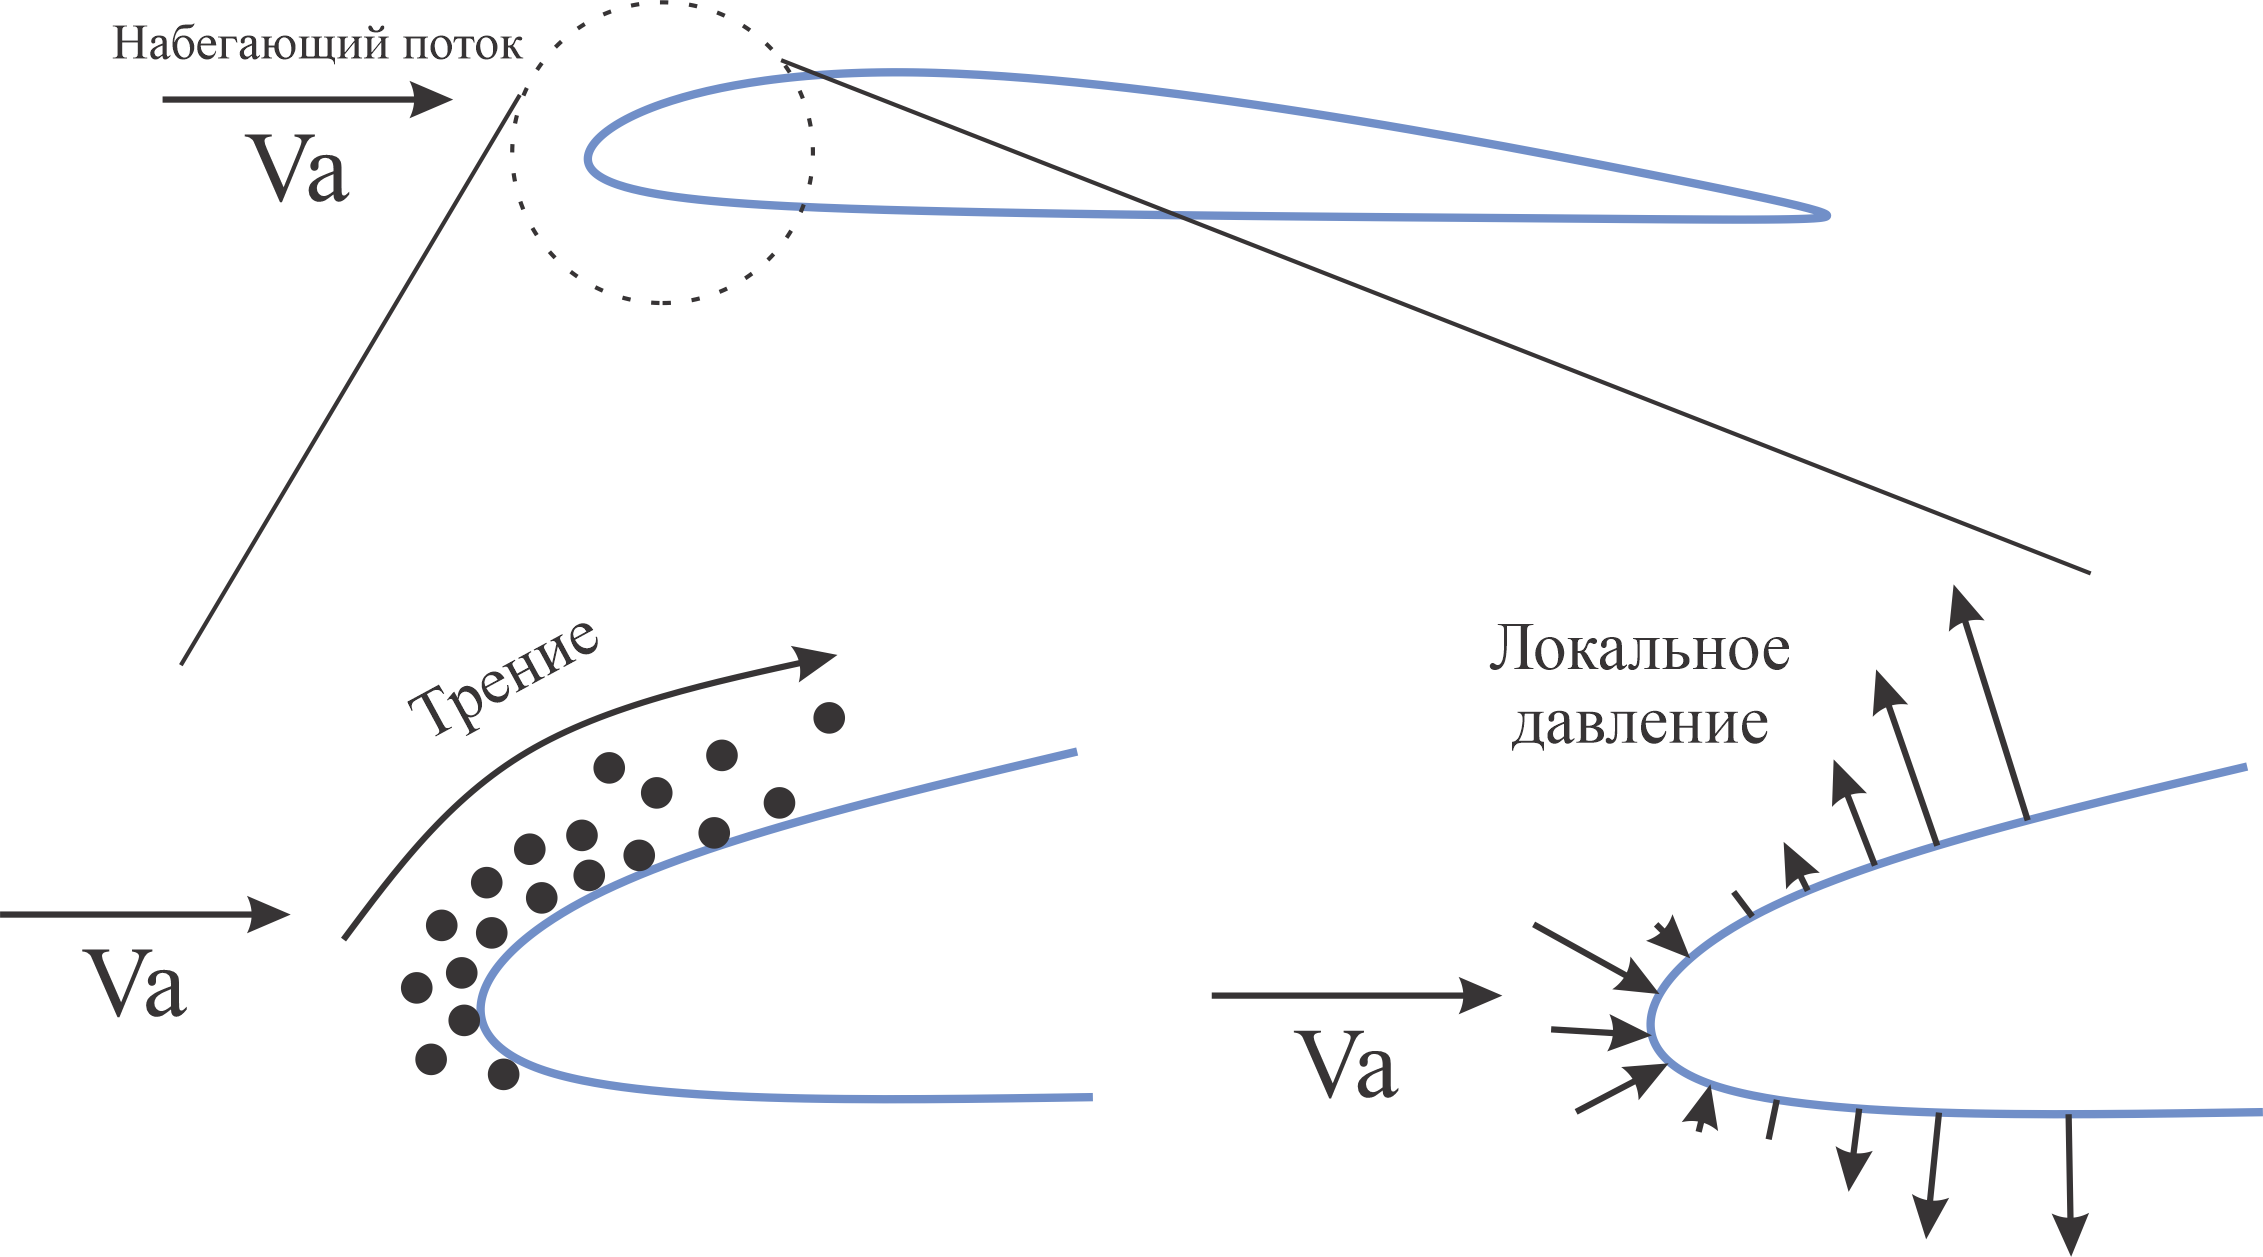
\includegraphics[width=0.8\linewidth]{DragForceSource.png}
	\end{figure}
}
%%%%%%%%%%%%%%%%%%%%%%%%%%%%%%%%%%%%%%%%%%%%%%
\only<2>{
	\small\justifying
	Сложный характер обтекания для качественных и инженерных методов оценки заменяют представлением сил и моментов сил через безразменые аэродинамические коэффициенты:
	$$
	\boldsymbol{f}_{aero} = QS\boldsymbol{C} = \frac{\rho V_a^2}{2}S\boldsymbol{C}(V, \alpha, \beta, \boldsymbol{\omega}^{b}_{b/i}, \boldsymbol{\delta}, ...),
	$$
	
	$Q = \frac{\rho V_a^2}{2}$ - динамический напор,\\
	$\boldsymbol{C}$ - аэродинамический коэффициент
}
%%%%%%%%%%%%%%%%%%%%%%%%%%%%%%%%%%%%%
\only<3>{
	В ветровой системе координат $F_w$ аэродинамические силы имеют простой вид
	\begin{columns}
		\column{0.5\textwidth}
			\begin{figure}
				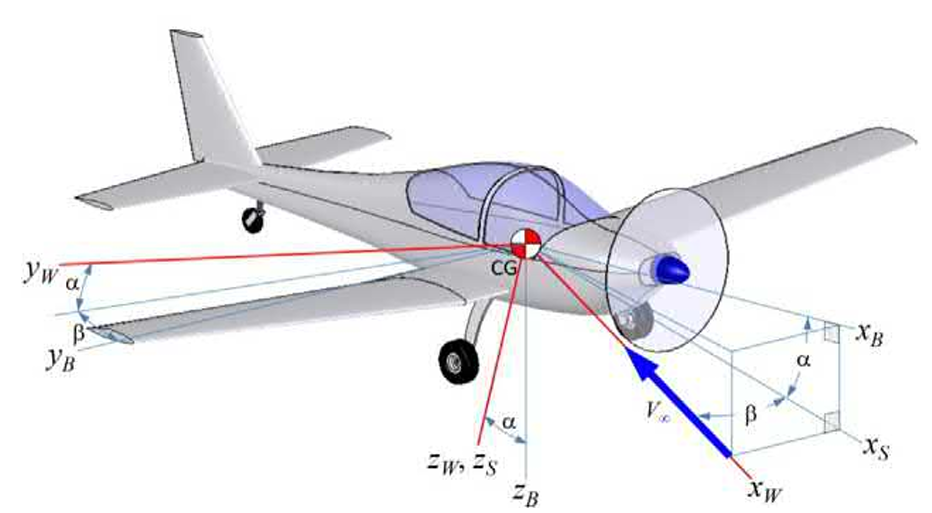
\includegraphics[width=1\linewidth]{WindAxis.png}
			\end{figure}
		\column{0.5\textwidth}
			$$R^w_b = R^w_s(\beta)\cdot R^s_b(-\alpha) = \\ 
			=\begin{pmatrix}
				c_\alpha & 0 & s_\alpha \\
				0 & 1 & 0 \\
				-s_\alpha & 0 & c_\alpha \\
			\end{pmatrix}
			\begin{pmatrix}
				c_\beta & s_\beta & 0 \\
				-s_\beta & c_\beta & 0 \\
				0 & 0 & 1 \\
			\end{pmatrix} = 
			\begin{pmatrix}
			c_\alpha c_\beta & s_\beta & s_\alpha c_\beta \\
			-c_\alpha s_\beta & c_\beta & -s_\alpha s_\beta\\
			-s_\alpha & 0 & c_\alpha\\ 
			\end{pmatrix}$$
	\end{columns}
}
%%%%%%%%%%%%%%%%%%%%%%%%%%%%%%%%%%%%%%%%%
\only<4>{
	\small\justifying
	Действуют три основных силы: лобового сопроивления, подъемная и боковая:
	$$
	\boldsymbol{f}^w_{aero} = \frac{\rho V^2_a}{2}S\begin{pmatrix}
		-C_D(V, \alpha, \beta, p, q, r, ...) \\ C_Y(V, \alpha, \beta, p, q, r, ...) \\ -C_L(V, \alpha, \beta, p, q, r, ...)\\
	\end{pmatrix}
	$$
	$C_D - \text{коэффициент лобового сопротивления}$\\
	$C_Y - \text{коэффициент боковой силы}$\\
	$C_L - \text{коэффициент подъемной силы}$	
}
\end{frame}
%%%%%%%%%%%%%%%%%%%%%%%%%%%%%%%%%%%%%%%%%%%%%%
\begin{frame}{Коэффициент подъемной силы $C_L$}
\only<1>{
	\small\justifying
	Каждый из коэффициентов можно разложить в ряд по параметрам в предположении малых величин. Пример коэффициента подъемной силы в общем случае:
	$$
	C_L = C_L_0 + \pdv{C_L}{\alpha}\alpha + \pdv{C_L}{\beta}\beta + \pdv{C_L}{p}p + \pdv{C_L}{q}q + \pdv{C_L}{r}r + \pdv{C_L}{\delta_{e}}\delta_{e} + \pdv{C_L}{\delta_{r}}\delta_{r} + \pdv{C_L}{\delta_{a}}\delta_{a}
	$$
	
	$$C_{()}_{x} - \text{производная аэродинамического коэффициента по параметру x}$$
	
	$$C_L = C_L_{0} + C_L_{\alpha}\alpha + C_L_{\beta}\beta + C_L_{p}p\frac{b}{2V_a} + C_L_{q}q\frac{c}{2V_a} + C_{L_{r}}r\frac{b}{2V_a} + C_{L_{\delta_e}}\delta_e + C_{L_{\delta_r}}\delta_r + C_{L_{\delta_a}}\delta_a$$
	$$C_{L_{\beta}} = C_{L_{p}} = C_{L_{r}} = C_{L_{\delta_{r}}} = C_{L_{\delta_a}} \approx 0$$
	\centering
	\boxed{
	C_L = C_L_{0} + C_L_{\alpha}\alpha + C_L_{q}q\frac{c}{2V_a} + C_L_{\delta_e}\delta_e
	}
}
%%%%%%%%%%%%%%%%%%%%%%%%%%%%%%%%%%%%%%%%%%%%%%
\only<2>{
	\begin{figure}
		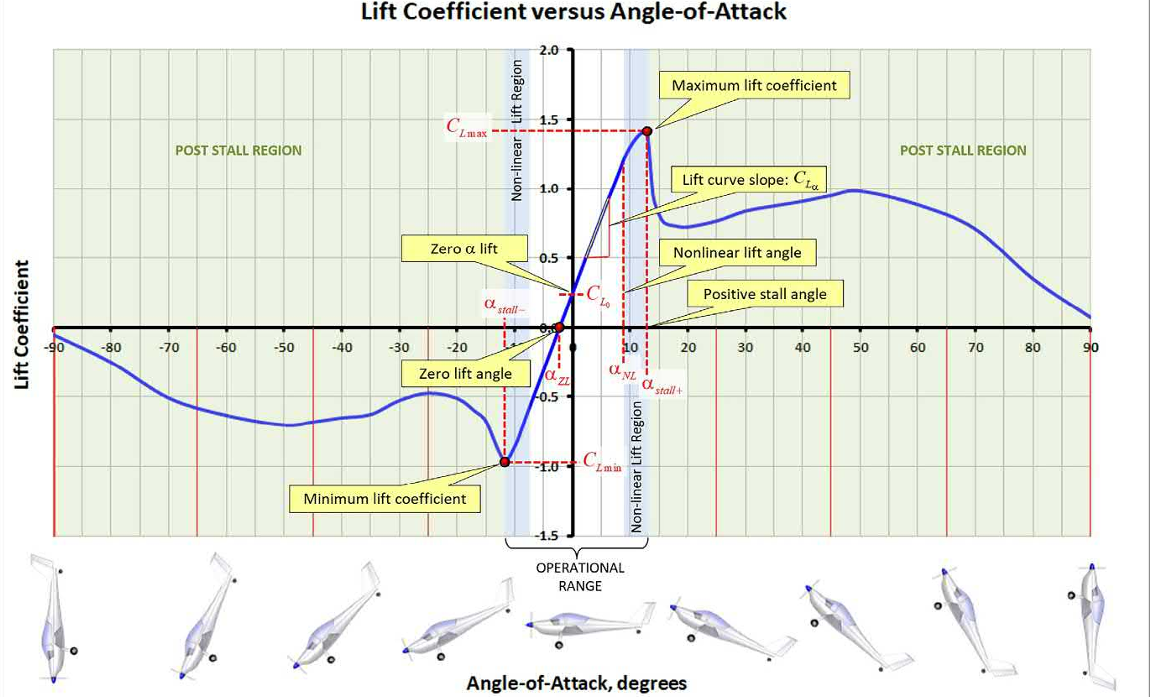
\includegraphics[width=0.9\linewidth]{LiftCurveRegions.png}
	\end{figure}
}
%%%%%%%%%%%%%%%%%%%%%%%%%%%%%%%%%%%%%%%%%%%%%%%%%%%%%%%%%%
\only<3>{
	\begin{figure}
		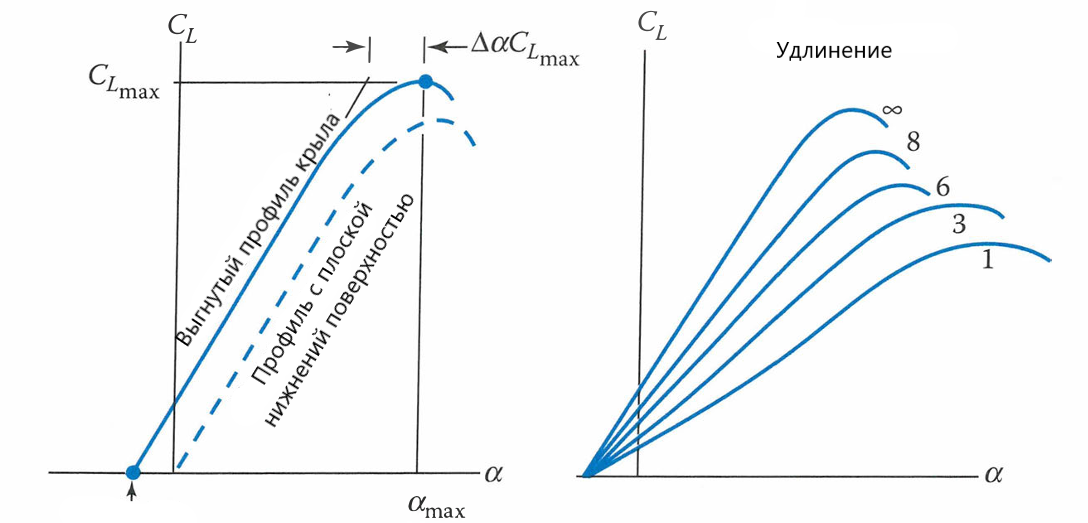
\includegraphics[width=1\linewidth]{LiftCurve.png}
	\end{figure}
}
\end{frame}
%%%%%%%%%%%%%%%%%%%%%%%%%%%%%%%%%%%%%%%%%%%%%%%%%%
\begin{frame}{Коэффициент лобового сопротивления}
	\only<1>{	
		\justifying\small
		$$
		C_D = C_D(\alpha) + C_{D_{\beta}}\beta + C_{D_{\delta_{e}}}\delta_{e} + C_{D_{\delta_{a}}}\delta_{a} + C_{D_{\delta_{r}}}\delta_{r} + ...
		$$
		По сравнению с $C_L$, $C_D$ имеет явно нелинейную зависимость от угла атаки. $C_{D}(\alpha) \propto \alpha^2$
		$$
		C_{D}(\alpha) = C_{D_{min}} + \frac{(C_{L} - C_{L_{minD}})^2}{A\pi e} = C_{D_{min}} + k(C_L - C_{L_{minD}})^2
		$$
		\centering
		\boxed{
		C_D = C_{D_{min}} + k(C_L - C_{L_{minD}})^2 + C_{D_{\beta}}\beta + C_{D_{\delta_{e}}}\delta_{e} + C_{D_{\delta_{a}}}\delta_{a} + C_{D_{\delta_{r}}}\delta_{r}
		}
	}
%%%%%%%%%%%%%%%%%%%%%%%%%%%%%%%%%%%%%%%%%%%%
\only<2>{
\begin{figure}
	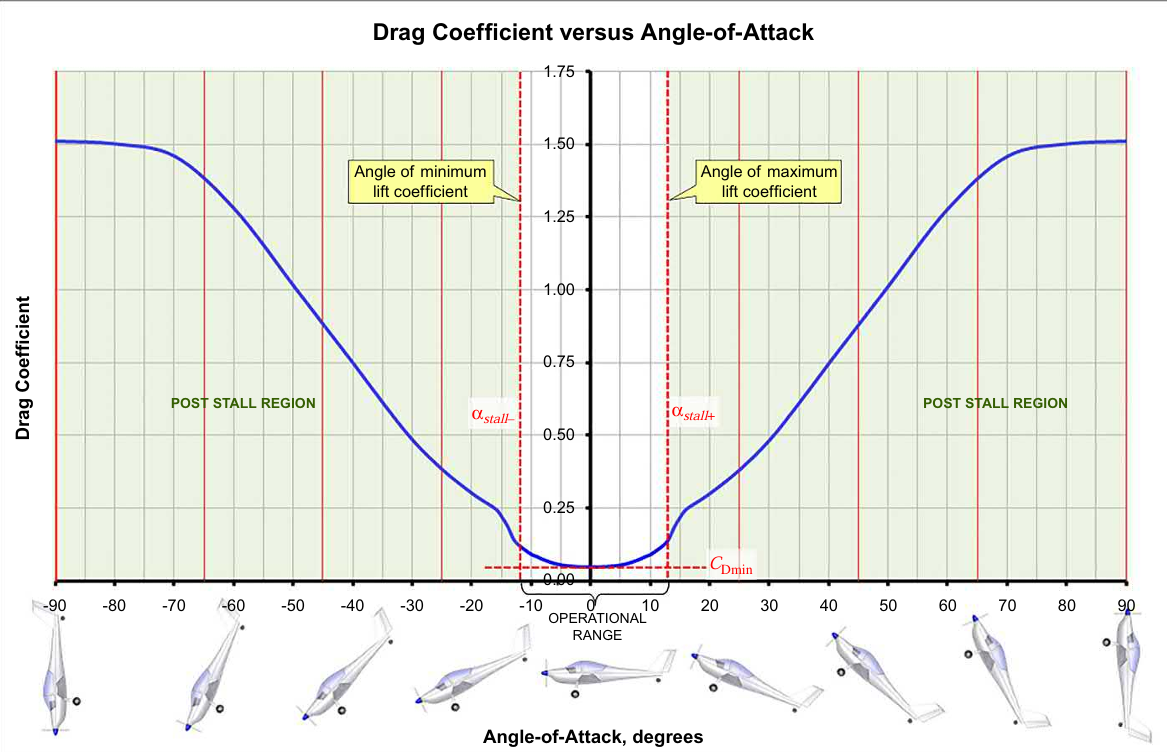
\includegraphics[width=0.85\linewidth]{DragVSAOA.png}
\end{figure}
}
%%%%%%%%%%%%%%%%%%%%%%%%%%%%%%%%%%%%%%%%%%%%%%%%
\only<3>{
	\begin{figure}
		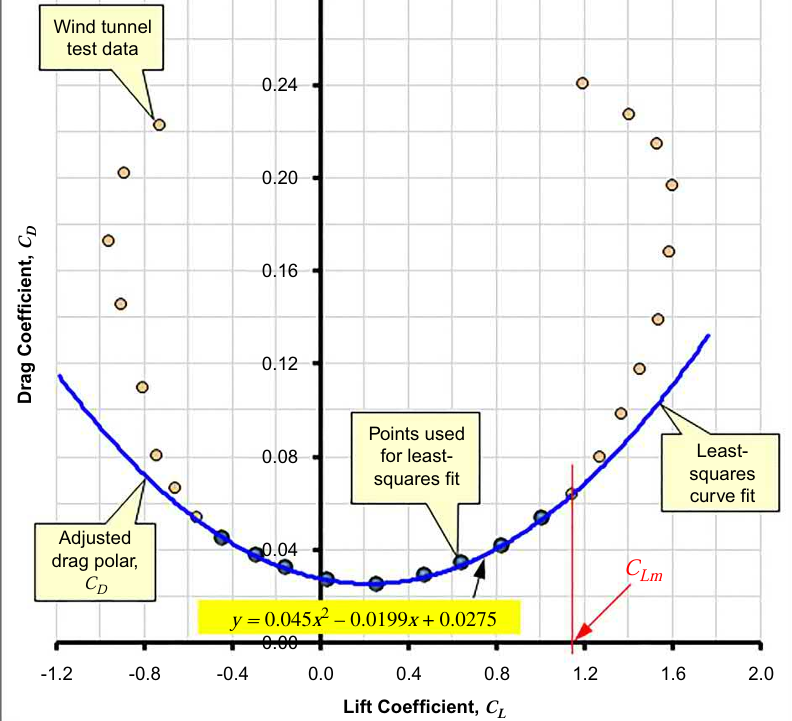
\includegraphics[width=0.6\linewidth]{DragPolar.png}
	\end{figure}
}
%%%%%%%%%%%%%%%%%%%%%%%%%%%%%%%%%%%%%%%%%%%%%%%%%%
\only<4>{
	\begin{columns}
		\column{0.5\textwidth}
		\begin{figure}
			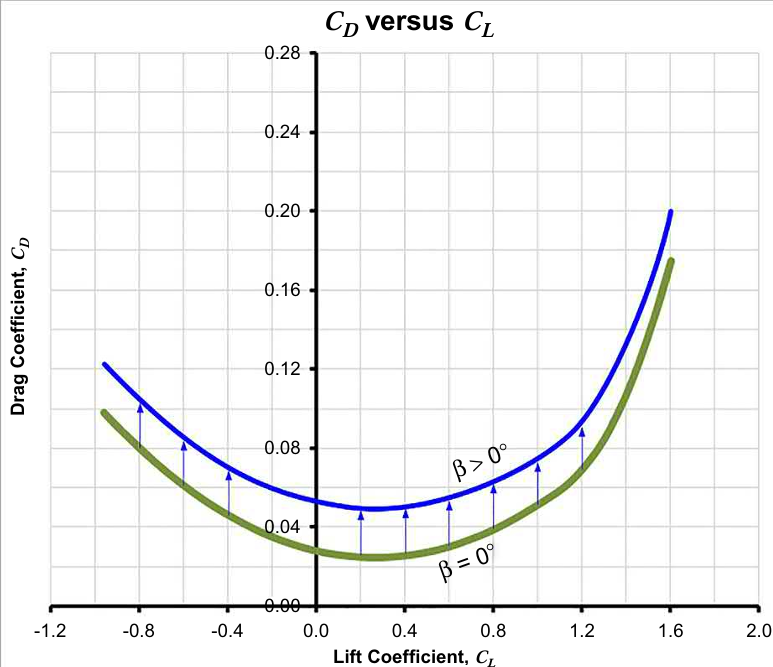
\includegraphics[width=1\linewidth]{DragVSBeta.png}
		\end{figure}
		\column{0.5\textwidth}
		\begin{figure}
			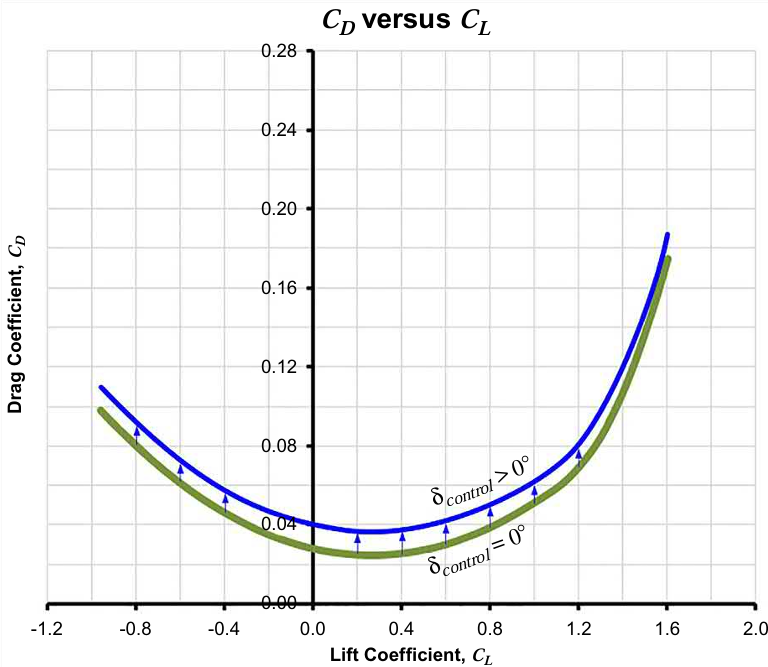
\includegraphics[width=1\linewidth]{DragVSControl.png}
		\end{figure}
	\end{columns}
}
\end{frame}
%%%%%%%%%%%%%%%%%%%%%%%%%%%%%%%%%%%%%%%%%%%%%%%%%%%%%%%%%%%%
\begin{frame}{Коэффициент боковой силы}
\only<1>{
	\justifying\small
	$$
	C_Y = C_{Y_{0}} + C_{Y_{\alpha}}\alpha + C_{Y_{\beta}}\beta + C_{Y_{\delta_{a}}}\delta_{a} + C_{Y_{\delta_{r}}}\delta_{r} + C_{Y_{p}}p\frac{b}{2V_a} + C_{Y_{r}}r\frac{b}{2V_a}
	$$
	Если ЛА симметричный то при стационарном горизонтальном полете боковой силы не возникает и $C_{Y_0} = C_{Y_{\alpha}} \approx 0$
	\centering
	\boxed{
	C_Y = C_{Y_{\beta}}\beta + C_{Y_{\delta_{a}}}\delta_{a} + C_{Y_{\delta_{r}}}\delta_{r}+ C_{Y_{p}}p\frac{b}{2V_a} + C_{Y_{r}}r\frac{b}{2V_a}
	}
	\begin{figure}
		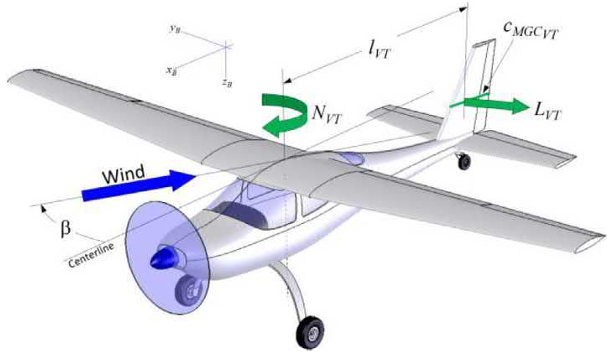
\includegraphics[width=0.5\textwidth]{SideForce.png}
	\end{figure}
}
%%%%%%%%%%%%%%%%%%%%%%%%%%%%%%%%%%%%%%%%%%%%%%%%%%
\only<2>{
	\begin{figure}
		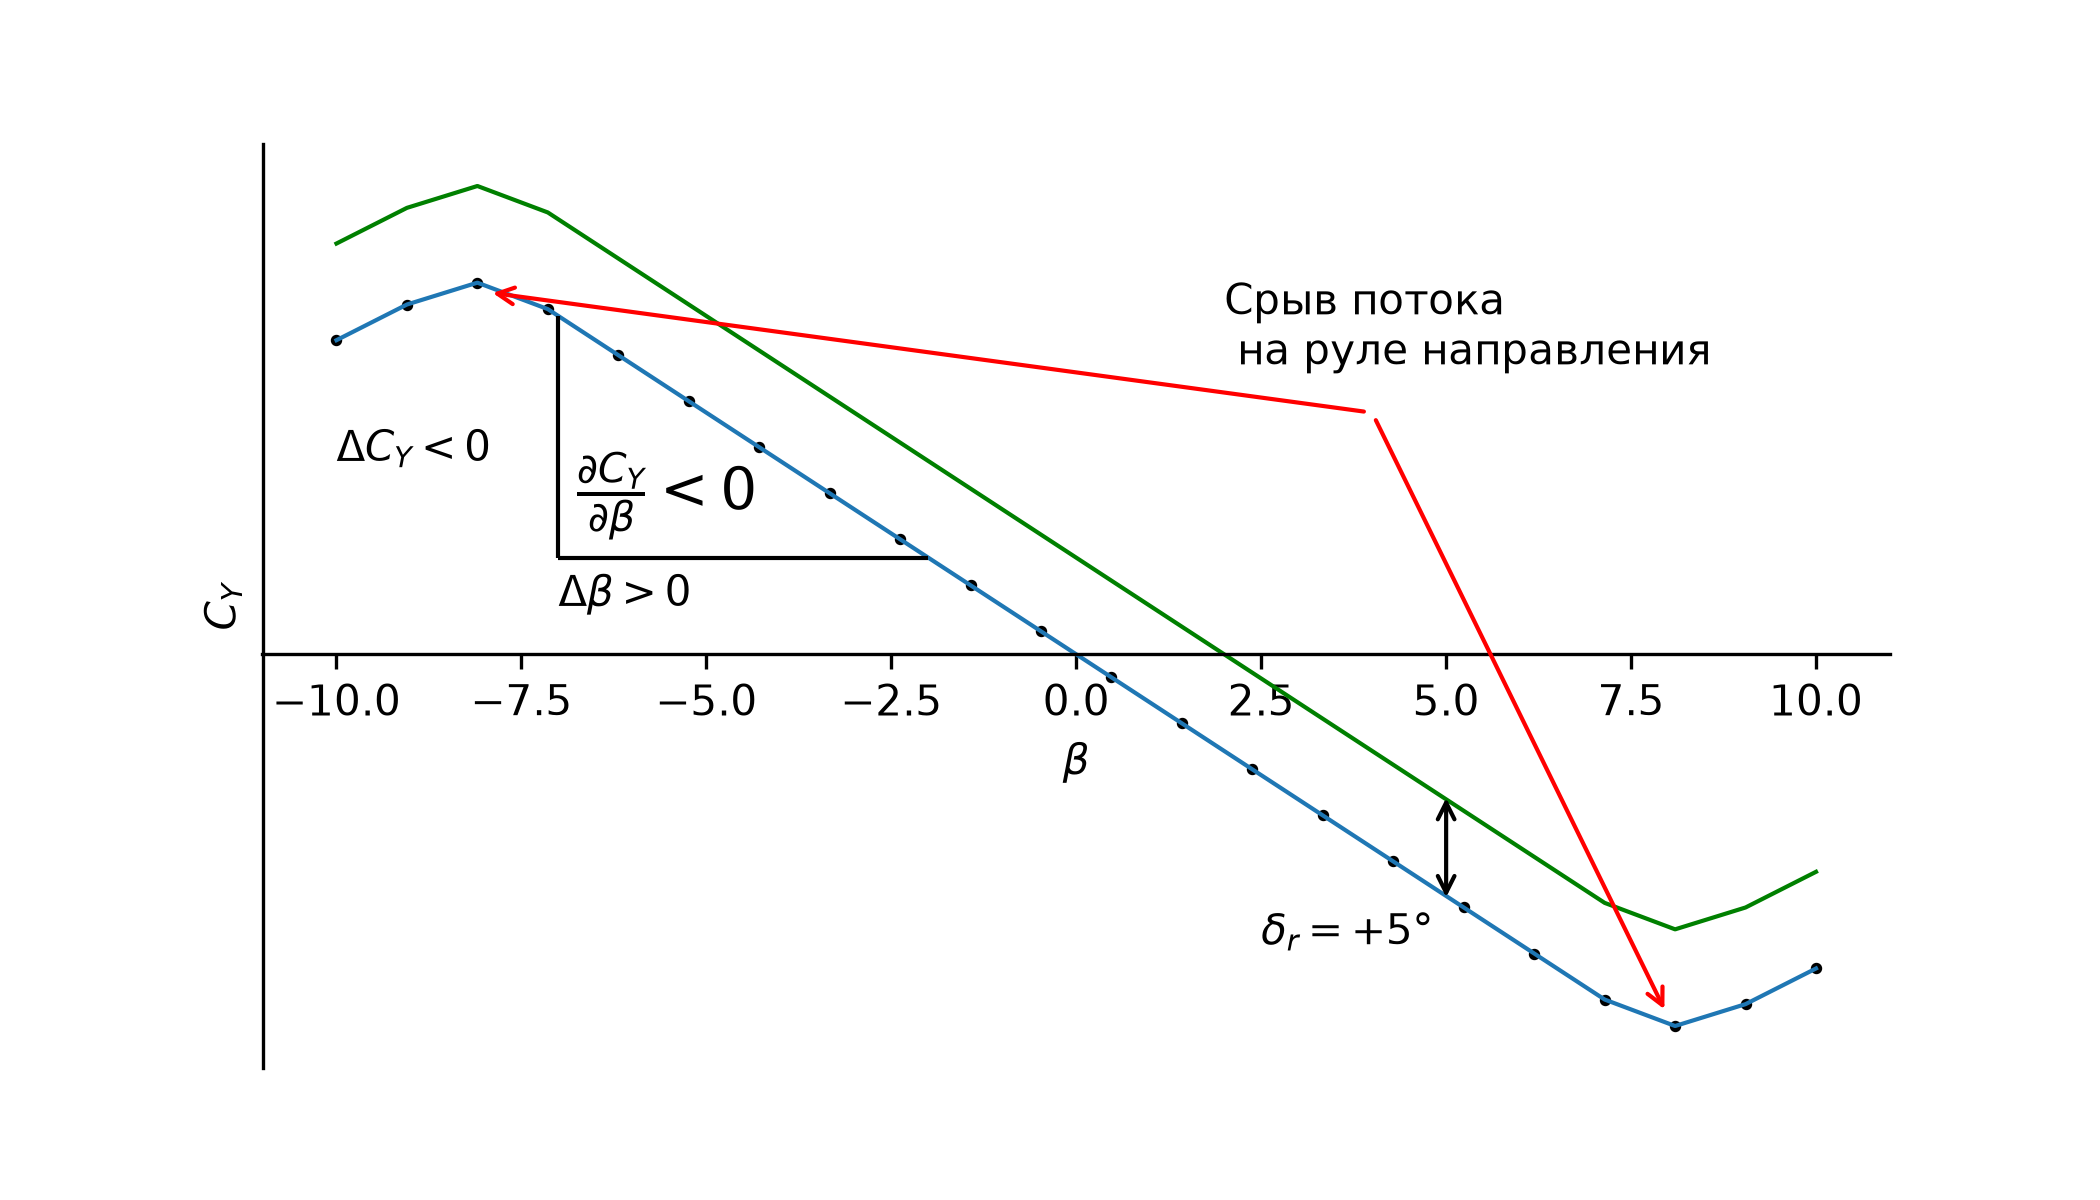
\includegraphics[width=1\textwidth]{CY(beta).png}
	\end{figure}
}
\end{frame}
%%%%%%%%%%%%%%%%%%%%%%%%%%%%%%%%%%%%%%%%%%%%%%%%%%%%%
\begin{frame}{Модель моментов сил}
	\justifying\small
	По аналогии с силами на ЛА действуют три момента, создаваемые аэродинамическими силами, которые в ветровой СК можно выразить как:
	$$
	\boldsymbol{M}^w_{aero} = \frac{\rho V^2_a}{2}S
	\begin{pmatrix}
		C_l b\\C_m c\\C_n b
	\end{pmatrix}
	$$ 
	$C_l - \text{коэффициент момента крена}$\\
	$C_m - \text{коэффициент момента тангажа}$\\
	$C_n - \text{коэффициент момента рыскания}$\\
	
	\centering
	\boxed{
		C_l = C_{l_0} + C_{l_{\beta}}\beta + C_{l_{p}}p\frac{b}{2V_a} + C_{l_{r}}r\frac{b}{2V_a} + C_{l_{\delta_{a}}}\delta_a + C_{l_{\delta_r}}\delta_r
	}
	\boxed{
		C_m = C_{m_0} + C_{m_{\alpha}}\alpha + C_{m_{\beta}}\beta + C_{m_{q}}q\frac{c}{2V_a} + C_{m_{\delta_{e}}}\delta_e
	}
	\boxed{
		C_n = C_{n_0} + C_{n_{\beta}}\beta + C_{n_{p}}p\frac{b}{2V_a} + C_{n_{r}}r\frac{b}{2V_a} + C_{n_{\delta_{r}}}\delta_r + C_{n_{\delta_r}}\delta_r
	}
	
\end{frame}
%%%%%%%%%%%%%%%%%%%%%%%%%%%%%%%%%%%%%%%%%%%%%%%%%%%
\begin{frame}{Коэффициент момента тангажа $C_m$}
	\only<1>{
	\begin{figure}
		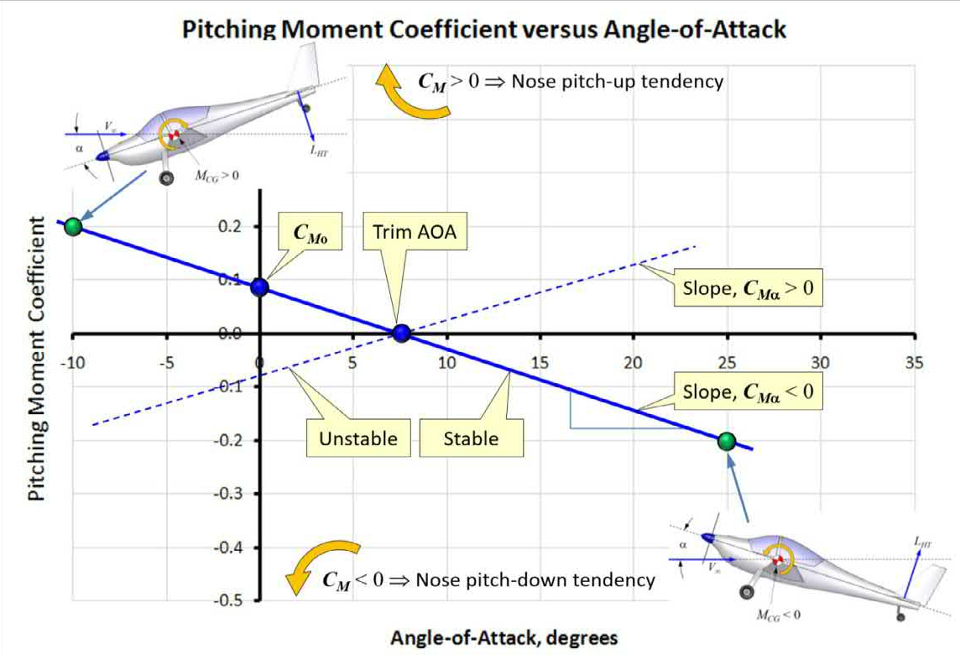
\includegraphics[width=0.8\textwidth]{CmVSAOA.png}
	\end{figure}
}
%%%%%%%%%%%%%%%%%%%%%%%%%%%%%%%%%%%%%%%%%%%%
\only<2>{
	\begin{columns}
		\column{0.6\textwidth}
			\begin{figure}
				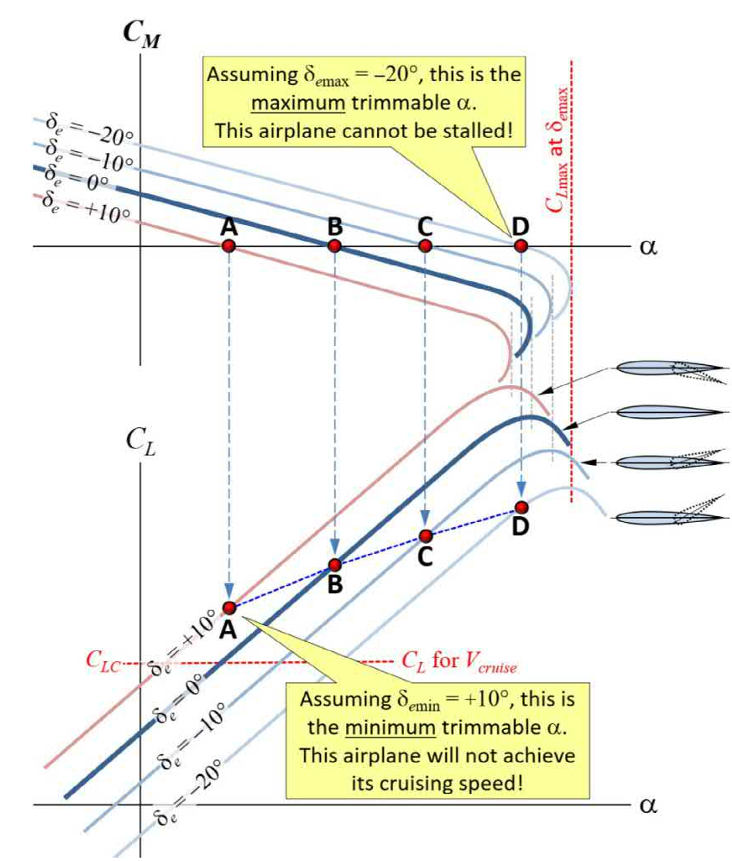
\includegraphics[width=0.78\textwidth]{CmVSCl.png}
			\end{figure}
			
		\column{0.4\textwidth}
		\justifying
			ЛА статически устойчив, если при отклонении от положения равновесия (подъем, опускание носа), момент тангажа возращает ЛА в положение устойчивого равновесия (горизонтальный полет):
			$$
			\pdv{C_m}{\alpha} = C_{m_{\alpha}} < 0
			$$
	\end{columns}

}
\end{frame}
%%%%%%%%%%%%%%%%%%%%%%%%%%%%%%%%%%%%%%%%%%%%%%%%%%%%%%%%
\begin{frame}{Коэффициент момента крена $C_l$}
	\begin{figure}
		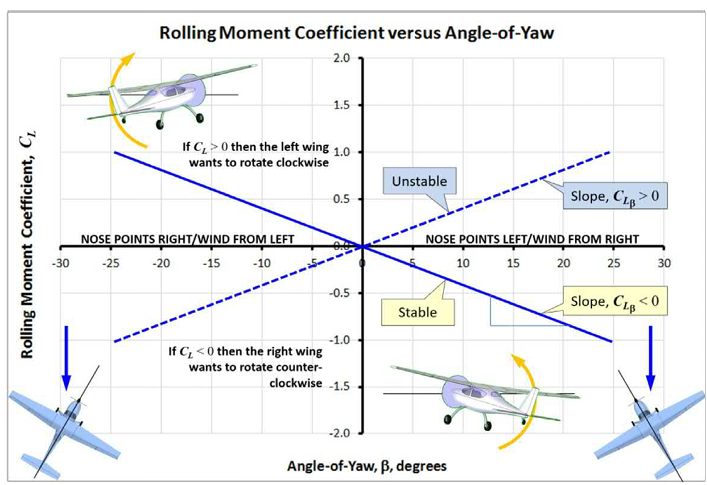
\includegraphics[width=0.8\linewidth]{ClVSBeta.png}
	\end{figure}
\end{frame}
%%%%%%%%%%%%%%%%%%%%%%%%%%%%%%%%%%%%%%%%%%%%%%%%%
\begin{frame}{Коэффициент момента рыскания $C_n$}
\only<1>{
	\begin{figure}
		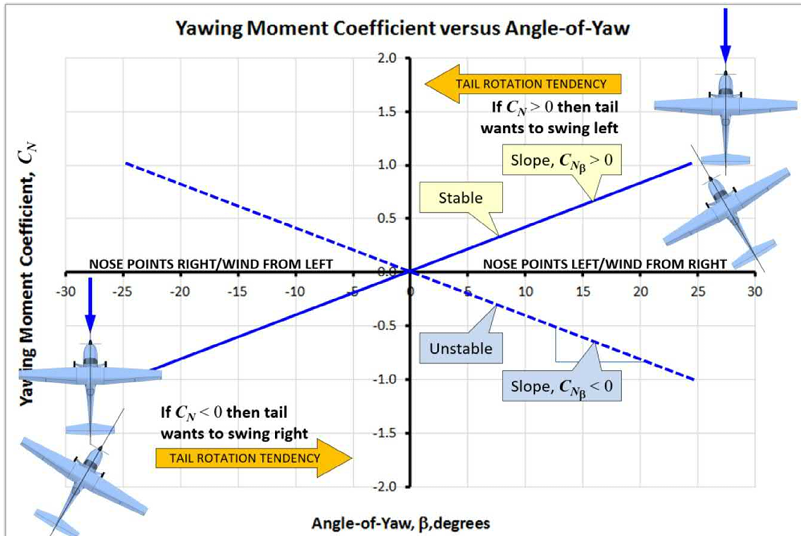
\includegraphics[width=0.8\linewidth]{CnVSBeta.png}
	\end{figure}
}
%%%%%%%%%%%%%%%%%%%%%%%%%%%%%%%%%%%%%%%
\only<2>{
	\begin{figure}
	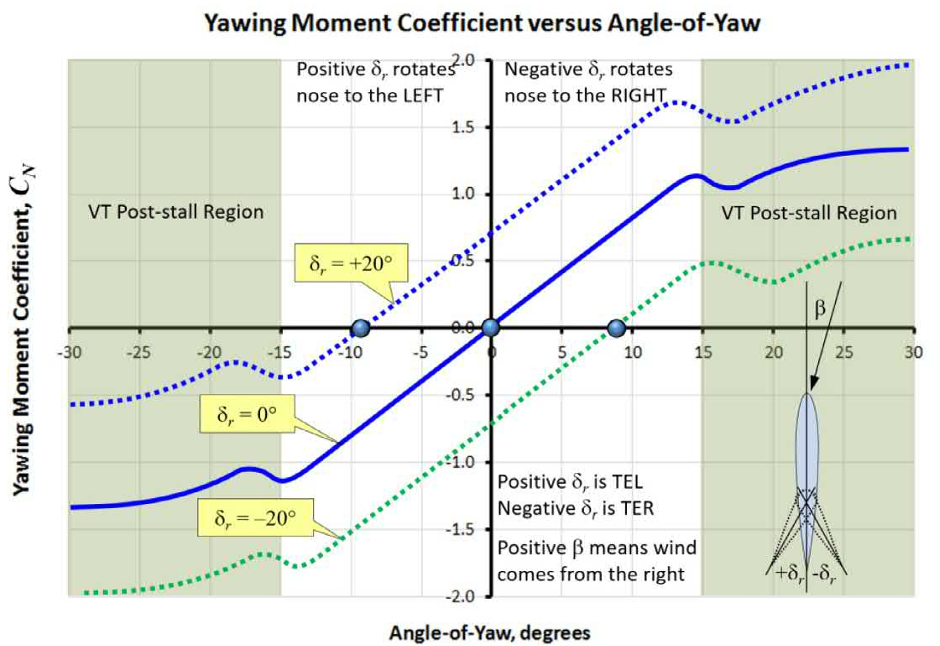
\includegraphics[width=0.8\linewidth]{CnVSControl.png}
	\end{figure}
}
\end{frame}
%%%%%%%%%%%%%%%%%%%%%%%%%%%%%%%%%%%%%%%%%%%%%
\begin{frame}{Силы и моменты аэродинамических сил в ССК}
	\justifying\small
	Все выкладки выше для аэродинамических сил и моментов относились к ветровой системе координат. В уравнениях движения ЛА силы и моменты выражены в ССК, поэтому матрицей поворота $R^b_w$ переведем $\boldsymbol{f}^w_{aero}$ и $\boldsymbol{M}^w_{aero}$ из ветровой СК в ССК:
	$$
	\boldsymbol{f}^b_{aero} = R^b_w\boldsymbol{f}^w_{aero} = \frac{\rho V^2_a}{2}S R^b_w
	\begin{pmatrix}
		-C_D\\ C_Y\\ -C_L\\
	\end{pmatrix}
	$$
	
	$$
	\boldsymbol{M}^b_{aero} = R^b_w\boldsymbol{M}^w_{aero} = \frac{\rho V^2_a}{2}S R^b_w
	\begin{pmatrix}
		C_l b\\ C_m c\\ C_n b\\
	\end{pmatrix}
	$$
\end{frame}
\end{document}
